\section{Final Product}
In diesem Kapitel wird das Ergebnis des Programmentwurfs durch mehrere Screenshots dargestellt.
\subsection{Klassenzimmer}
\begin{figure}[H]
  \centering
  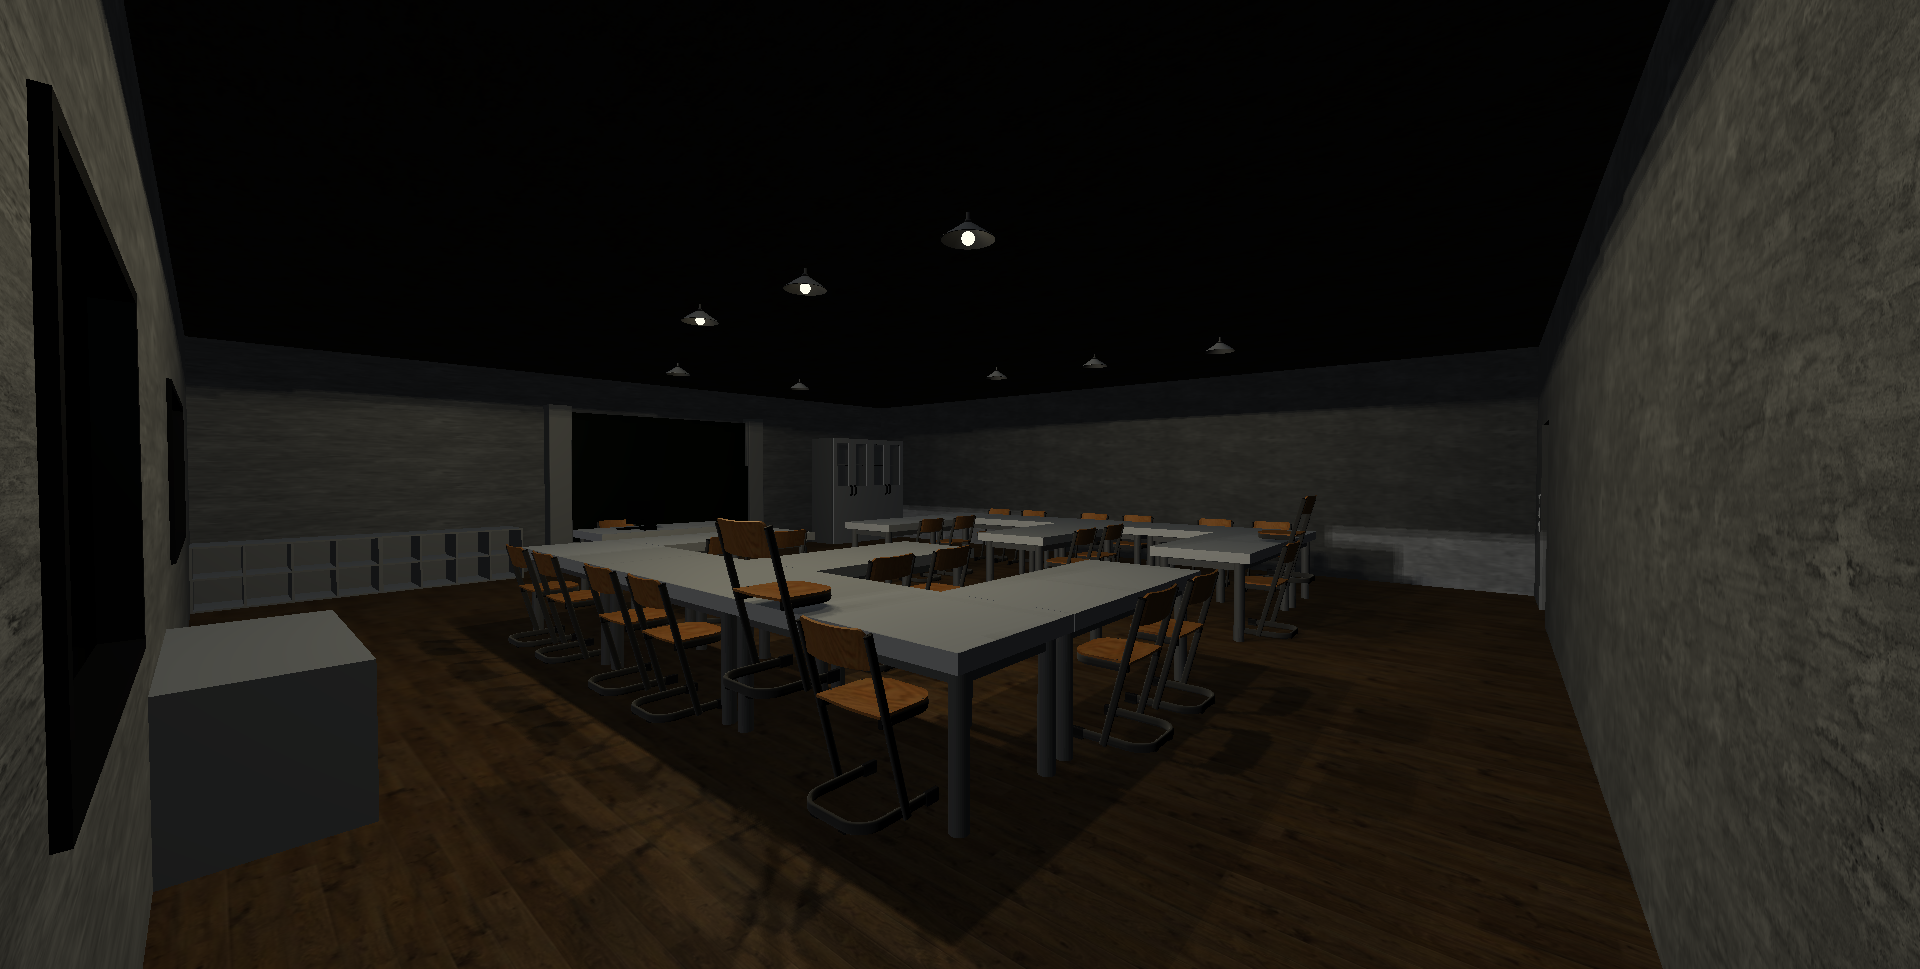
\includegraphics[width=1\textwidth]{images/finalproduct/screenshot_all_shader_only_one_lamp.png}
  \caption{Klassenzimmer nur ein Lampencluster}
  \label{fig:ScreenshotShaderOneLamp}
\end{figure}\noindent
\begin{figure}[H]
  \centering
  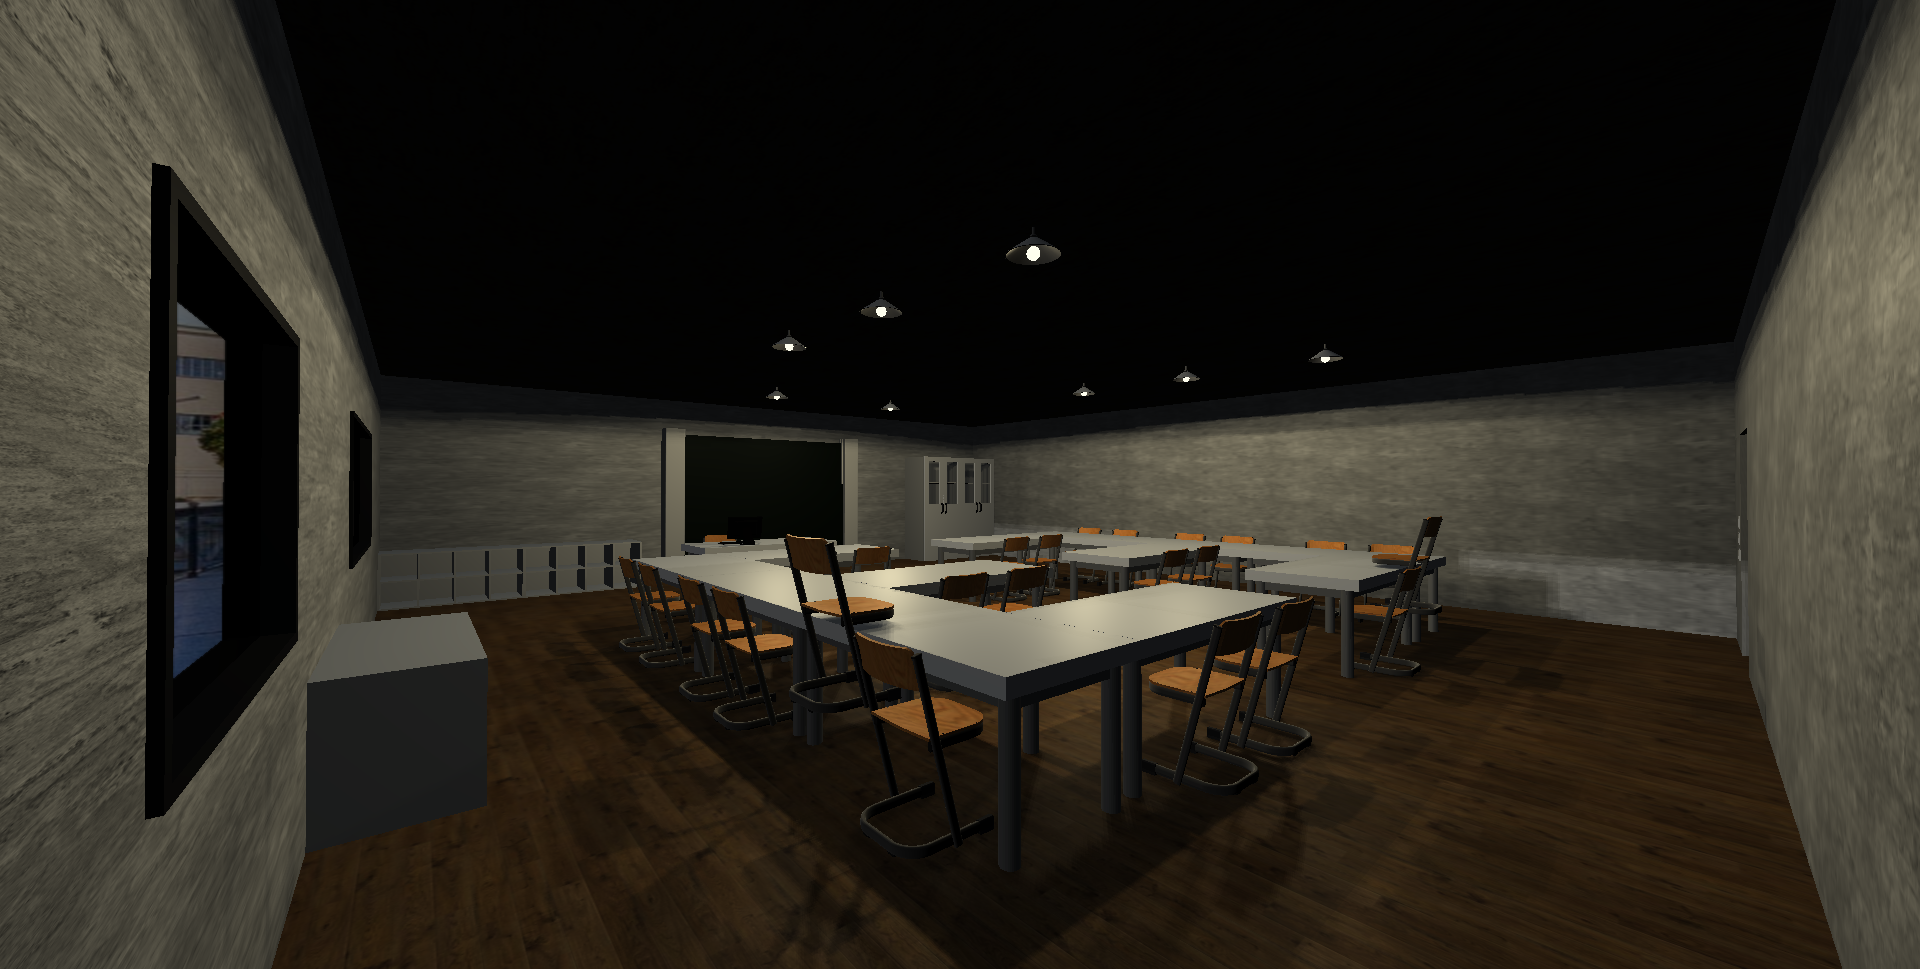
\includegraphics[width=1\textwidth]{images/finalproduct/screenshot_all_shader.png}
  \caption{Klassenzimmer alle Lampen}
  \label{fig:ScreenshotShaderAllLamp}
\end{figure}\noindent
\begin{figure}[H]
  \centering
  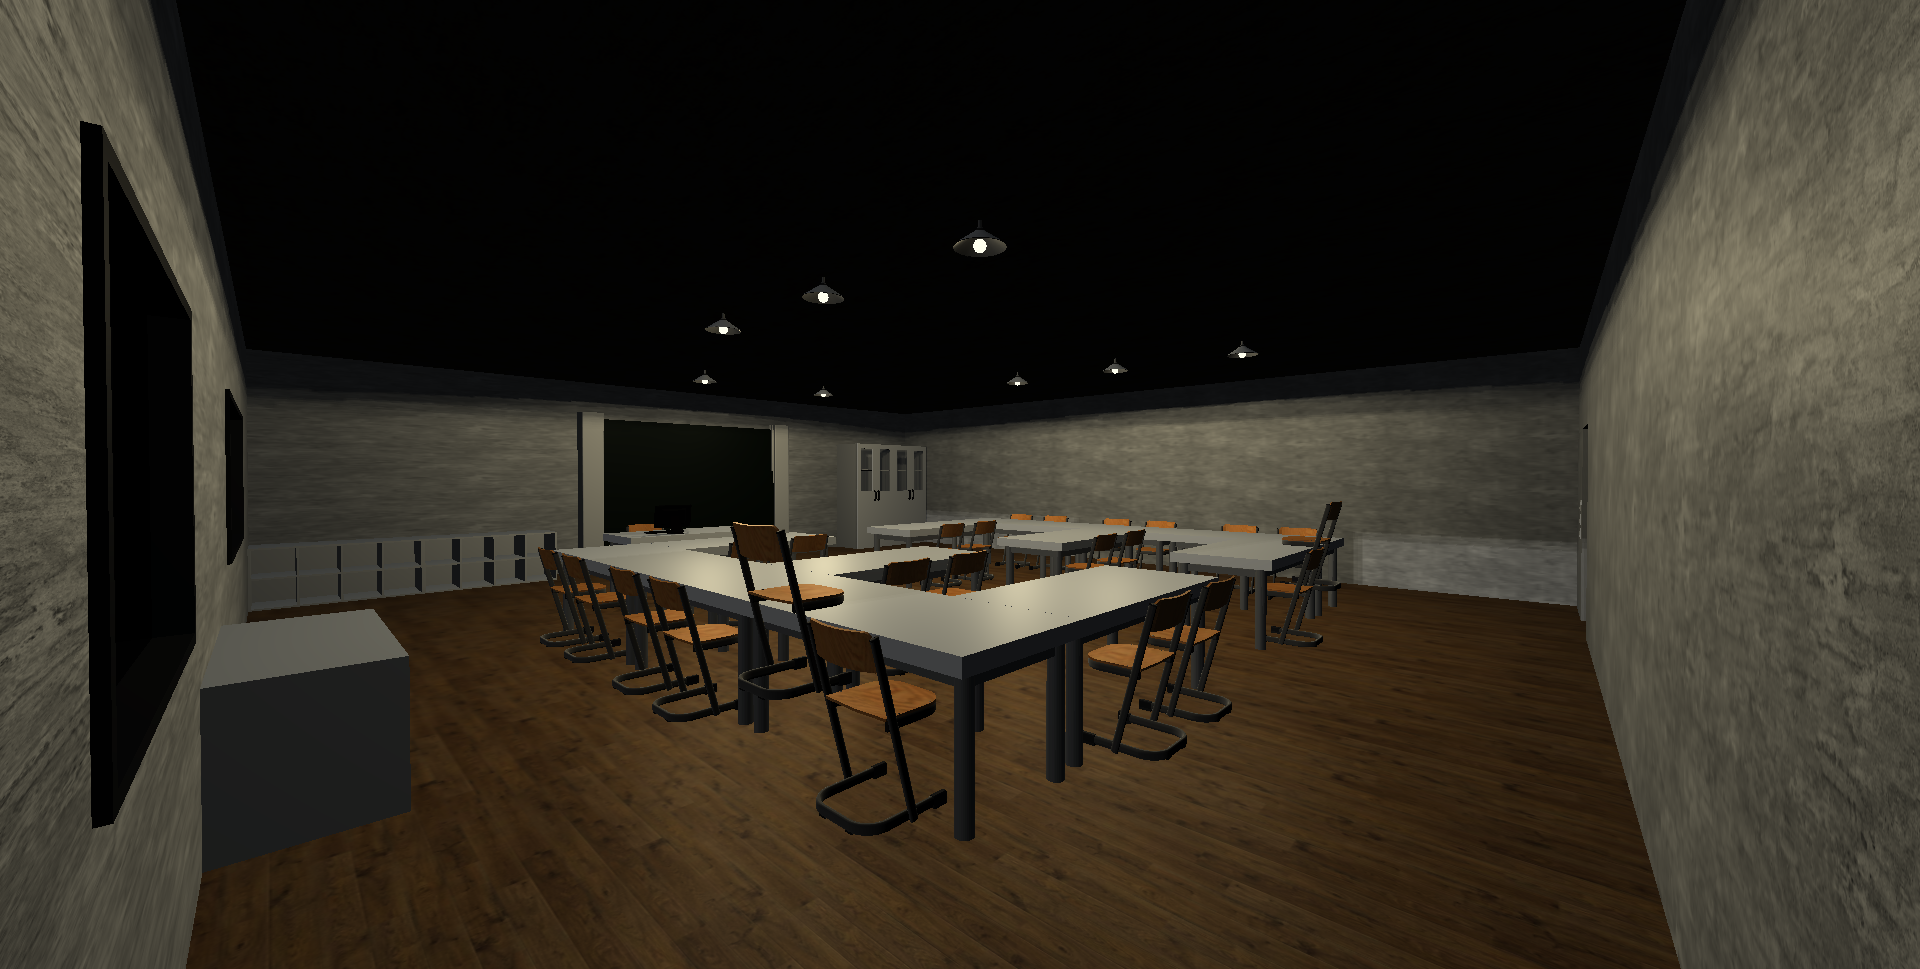
\includegraphics[width=1\textwidth]{images/finalproduct/screenshot_no_shader.png}
  \caption{Klassenzimmer ohne Schatten}
  \label{fig:ScreenshotNoShaderAllLamp}
\end{figure}\noindent
\subsection{Flugsimulator}
\begin{figure}[H]
  \centering
  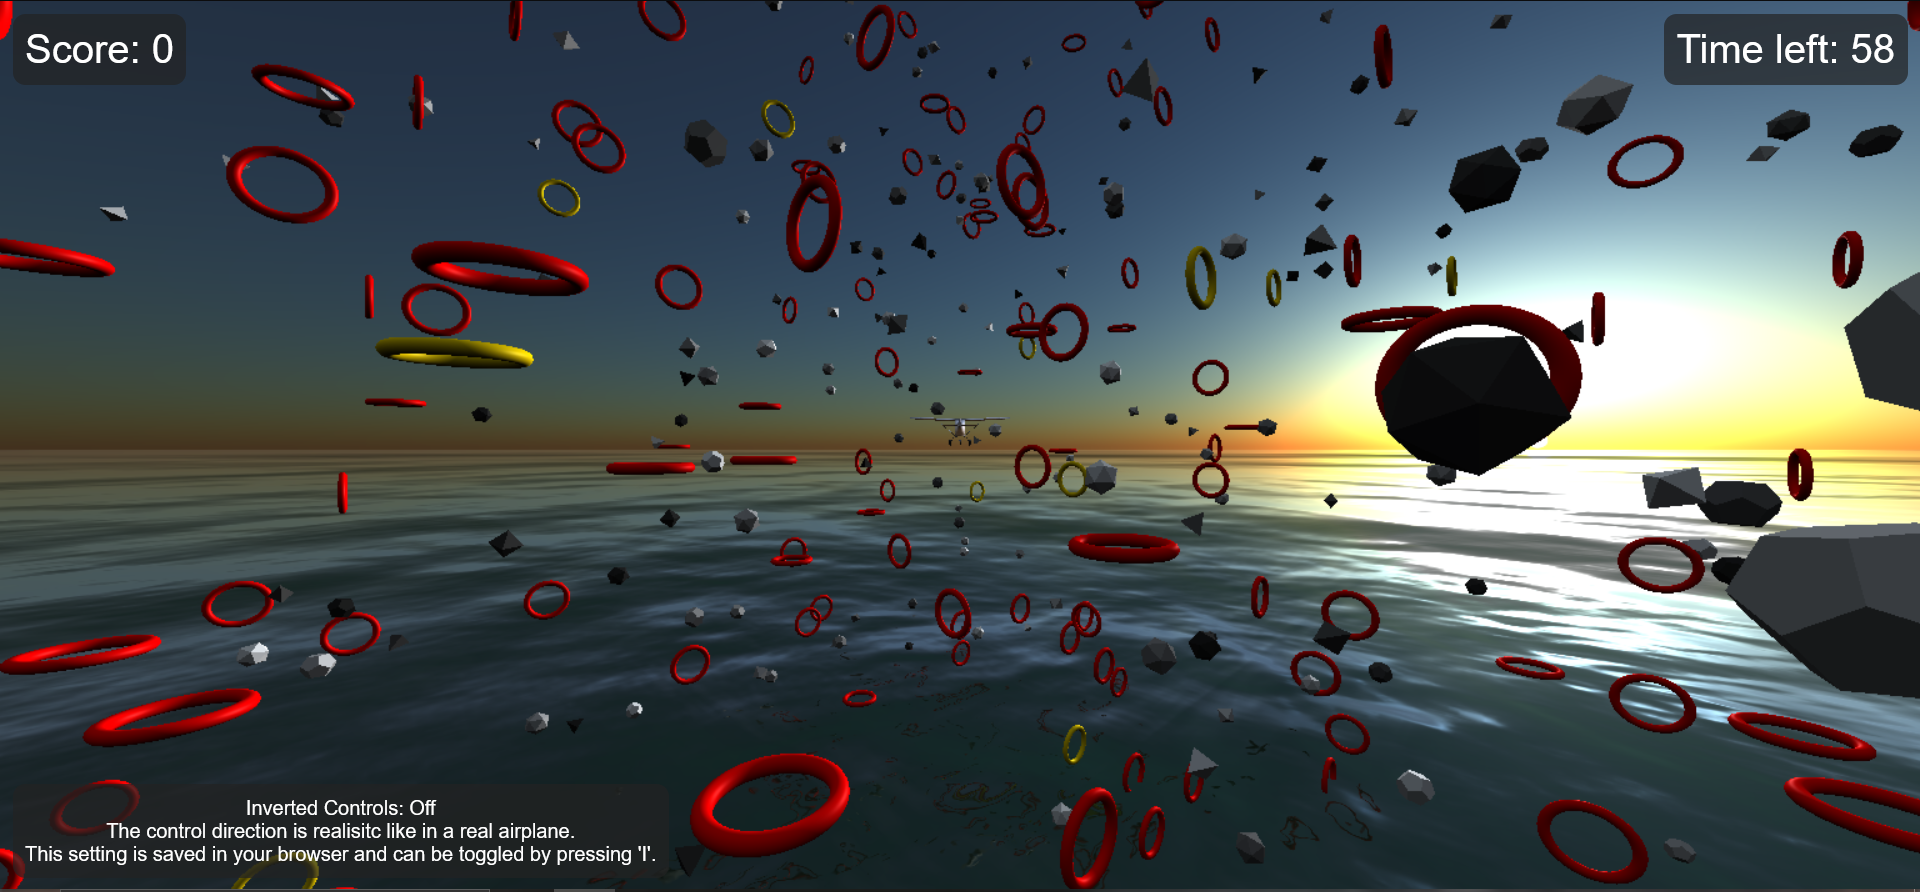
\includegraphics[width=1\textwidth]{images/finalproduct/screenshot_flightsim.png}
  \caption{Flugsimulator}
  \label{fig:ScreenshotFlightSim}
\end{figure}\noindent
\begin{figure}[H]
  \centering
  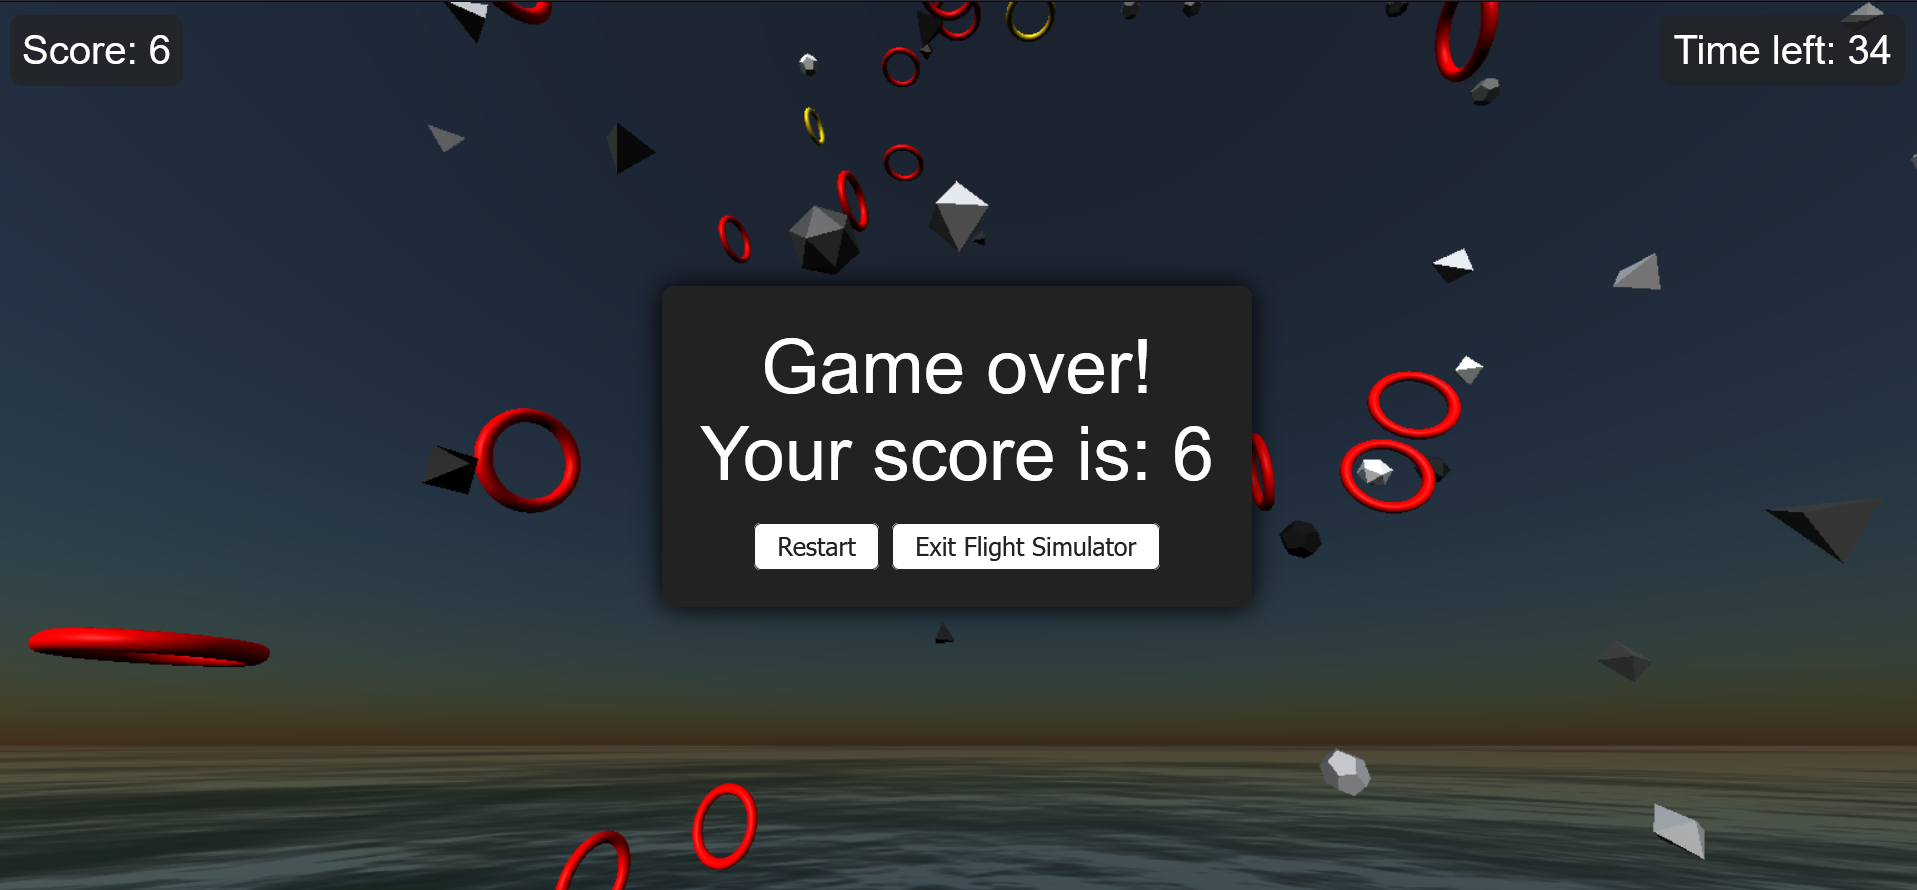
\includegraphics[width=1\textwidth]{images/finalproduct/screenshot_flightsim_score.png}
  \caption{Flugsimulator Game Over}
  \label{fig:ScreenshotFlightSimScore}
\end{figure}\noindent